
\section{Running the MSTransform framework}\label{Sec:Running}

%\htmladdnormallink{These slides}{http://www.aoc.nrao.edu/~rurvashi/DataFiles/Talk_FlaggingCASA3.4.pdf}
Summarize the CASA MSTransform infrastructure and user-options.

\htmladdnormallink{Task Documentation}{http://casa.nrao.edu/docs/TaskRef/TaskRef.html}
\htmladdnormallink{Tool Documentation} {http://casa.nrao.edu/docs/CasaRef/CasaRef.html}

\subsection{Notes during development}
These notes should become part of the real documentation later. For the moment they are
only notes to remind me of details of the implementation.

\begin{environment}
\item phasecenter: (int) or (str). As int, it gives the FIELD ID for the mosaic center. If a string,
it gives the center coordinate, e.g. 'J2000 12h56m43.88s +21d41m00.1s'. Default is '', which means, the 
first selected field.
\item cvel: if the regridding parameters are left untouched and a spw selection is given, cvel will always
combine the spws. When passall=False, it will save to the output only the combined spw. If passall=true,
it will save the combined spws and copy the other spws to the output too. In mstransform, only
the passall=false behaviour is supported.

Cvel always combines spws!
\item Even when combinespws=False, the selected spws will be re-indexed in the output.
\item Hanning: the behavior will be the following: Hanning will be applied to all the datacolumns
requested by the user in the parameter 'datacolumn'. If the requested column does not exist,
it will be an error. This is different of what the hanningsmooth task currently does.
\item Depending on the separationaxis selected for partition, some transformation cannot
be performed. These cases are caught in the beginning of the processing.
separation   combinespws  separatespws  regridms  freqaverage  timespan  hanning
axis
---------------------------------------------------------------------------------------
spw            NO           YES*         YES        YES          YES       YES
scan           YES          YES          YES        YES          YES**     YES
both           NO           YES*         YES        YES          NO        YES

REVIEW the following cases
*  --> we can separate spws when separationaxis='spw' only if run in sequential.
** --> we can partition per scan but cannot let timebins span changes in scan, which
       is one of the parameters of the timeaverage transformation.
\item 
\item 
\end{environment}











%%%%%%%%%%%%%%%%%%%%%%%%%%%%%%%%%%%%%%%%%%%%%%%%%%%%

\subsection{Single flag mode (flagdata)}

All the following flagging modes operate on user-specified subsets of the data.
The dataset is iterated-through in chunks consisting of one field, one spw, and a
user-defined timerange (default is one scan). 
Modes that read visibilities also respond to some simple expressions that are applied to 
the visibilities, before they are considered for flagging 
(for example, $ABS\_RR,LL,  ABS\_I, REAL\_V,  ABS\_ALL$).


\subsubsection{Shadow}

Shadow flags are computed by considering the positions and diameters of a list of antennas
along with the target direction at each timestep.  
All antennas present in the ANTENNA subtable of the MS as well as any other positions 
and diameters supplied via an external file are considered for shadow-flag calculations. 

Shadow flags are computed as follows (for every timestep): 
\begin{enumerate}
\item Calculate or read the $u,v,w$ values (in meters) for all possible antenna-pairs, 
using the phase-reference center of the observation to define the pointing-direction. 
The values of $u,v,w$ are re-used when already present in the MS, and calculated only for
baselines without visibilities in the current timestep (to account for antennas that did not produce
data for that timestep, but were still physically present and creating shadows).

\end{enumerate}


\begin{figure}
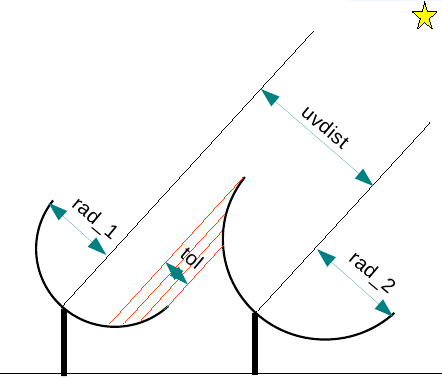
\includegraphics[scale=0.7]{shadow.diagram.png}
\caption{This figure shows the geometry used to compute shadowed antennas.}
\end{figure}



Note : The use of the phase-reference center as the pointing-direction for all antennas, is accurate in most 
cases, but will be approximate during on-the-fly mosaicing. However, since it is unlikely that an 
on-the-fly mosaic will be done with only one phase-reference center on a large-enough field-of-view
for shadow-flag differences to become significant.  


Note : Antennas that are not part of the MS ANTENNA subtable can be included in the calculation of
shadow flags by specifying a list of positions and diameters in an external file.   Note however that
the calculations will not account for the fact that antennas not part of
the observation, but still physically present on the ground, may not be pointing in the same direction as all the others
(as is assumed in the calculations).  If desired, the antenna diameters in the external file could
be adjusted accordingly.

Example : 
\begin{verbatim}
name=VLA1
diameter=25.0
Position=[-1601144.96146, -5041998.01971, 3554864.76811]

name=VLA2
diameter=25.0
position=[-1601105.76646, -5042022.39178, 3554847.24515]
\end{verbatim}

A helper-function has been provided to construct this list from an MS (possibly a different dataset)
that contains the required information in its ANTENNA subtable.

\begin{verbatim}
import flaghelper;
antlist =  flaghelper.extractAntennaInfo (
            msname='shadowtest.ms',
            antnamelist=['VLA1','VLA2','VLA9','VLA10'] );
flaghelper.writeAntennaList('antlist.txt',antlist);
\end{verbatim}


Figure \ref{ShadowExample} shows the flagging results from a simulated observation that spans a large
elevation range. Antennas near the center of the array are shadowed more than the others (left plot). 
If some antennas are split-out of the dataset, the ANTENNA subtable will have fewer antennas, and the shadow
flags will change (middle plot).  However, by specifying the positions and diameters of the missing antennas
via the external file, the correct shadow flags are recovered (right plot). 

\begin{figure}
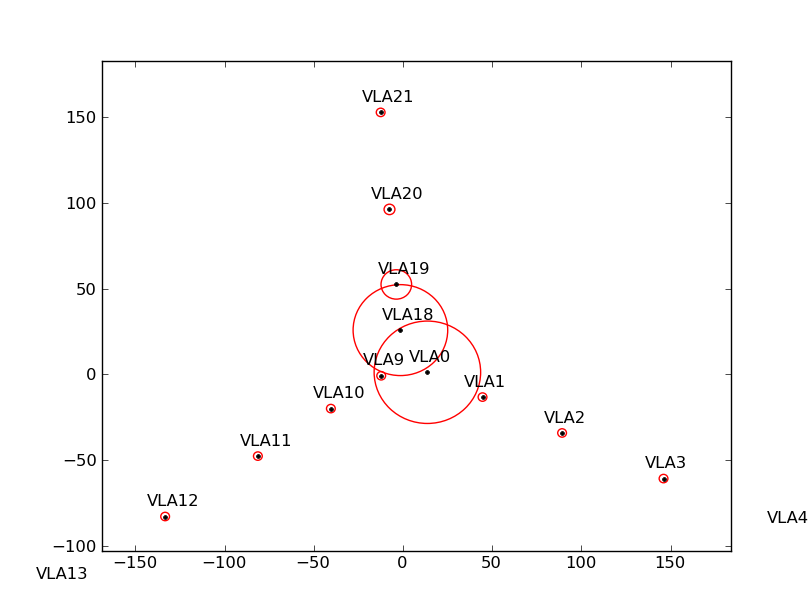
\includegraphics[scale=0.5]{plot.allants.shadow.png}
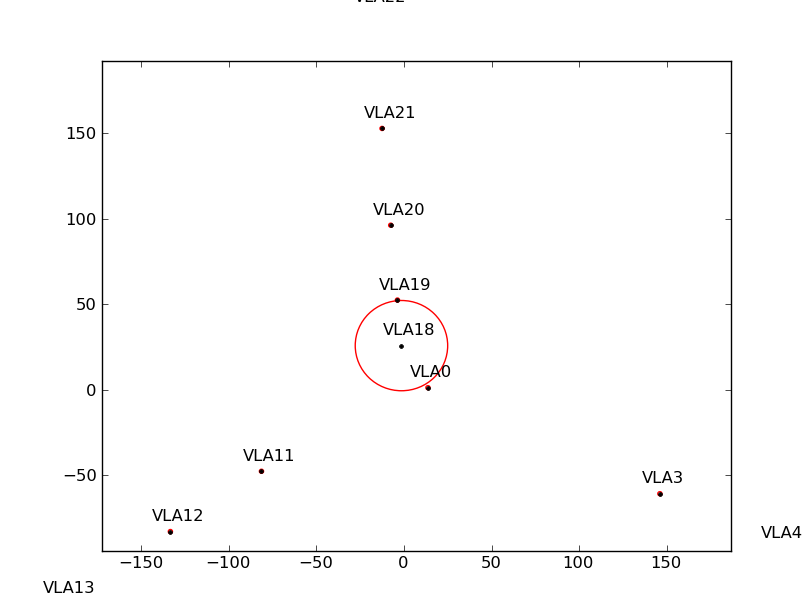
\includegraphics[scale=0.5]{plot.someants.shadow.png}
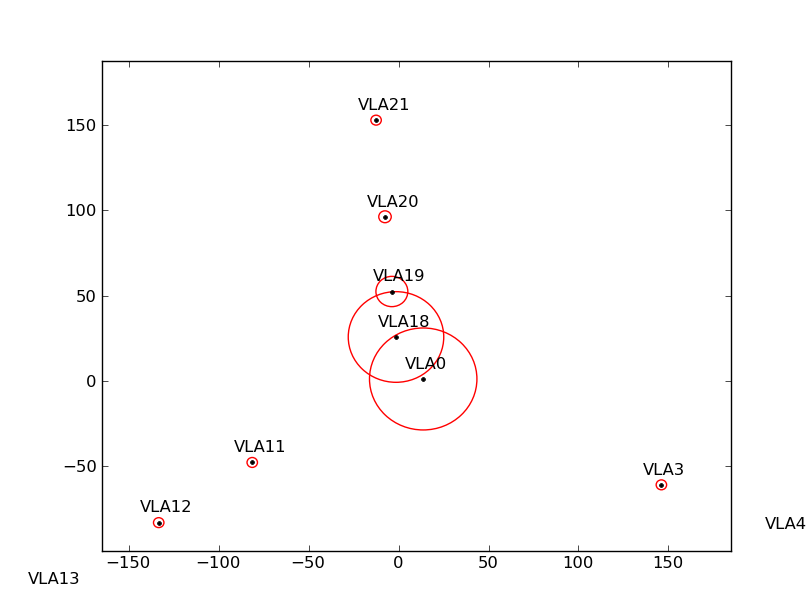
\includegraphics[scale=0.5]{plot.someants.withlist.shadow.png}
\caption{This figure shows  fractions of data flagged per antenna, for
three different use-cases. The size of the circle is proportional to the fraction of data flagged.
(LEFT) : Shadow-Flags with all antennas present in the MS,   (MIDDLE) : Shadow-Flags with four antennas (and their baselines) deleted from the MS,    (RIGHT) : Shadow-Flags from the MS with the missing antennas, but with the positions and diameters of the missing antennas specified via an external text file. The flags produced are the same as when all antennas are present in the MS.}
\label{Fig:ShadowExample}
\end{figure}


\subsubsection{TFCrop}

TFCrop is an autoflag algorithm that detects outliers on the 2D time-frequency plane, and 
 can operate on un-calibrated data (non bandpass-corrected).

The original implementation of this algorithm is described in 
\htmladdnormallink{NCRA Technical Report 202}{http://ncralib1.ncra.tifr.res.in:8080/jspui/handle/2301/127} (Oct 2003)


The algorithm iterates through the data in chunks of time.
For each chunk,  the result of user-specified visibility-expressions 
are organized as 2D time-frequency planes, one for each baseline 
and correlation-expression result, and the following steps are performed.

\begin{enumerate}
\item Calculate a bandshape template : 
Average the data across time, to construct an average bandpass.
     Construct an estimate of a clean bandpass (without RFI) via a
     robust piece-wise polynomial fit to the average bandpass shape.

       Note : A robust fit is computed in upto 5 iterations. 
It begins with a straight line fit across the full range, and gradually increases to 
     'maxnpieces' number of pieces with third-order polynomials in each piece. 
At each iteration, the stddev
                                between the data and the fit is computed, values beyond N-stddev are flagged,
                                and the fit and stddev are re-calculated with the remaining points.
                                This stddev calculation is adaptive, and converges to a value that reflects 
                                only the data and no RFI.  
At each iteration,  the same relative threshold is applied to detect flags, and this results in
a varying set of flagging thresholds,  that allows deep flagging only when the fit represents the true data best.
 Iterations stop when the stddev changes 
     by less than 10\%, or when 5 iterations are completed.

     The resulting clean bandpass is a fit across the base of RFI spikes.

\item  Divide out this clean bandpass function from all timesteps in the current chunk.  
Now, any data points that deviate from a mean of 1 can be considered RFI.  This step 
helps to separate narrow-band RFI spikes from a smooth but varying bandpass, in
situations where a simple range-based clipping will flag good sections of the bandpass.

\item Perform iterative flagging (robust flagging) of points deviating from a value of 1.  

  Flagging is done in upto 5 iterations. 
   In each iteration, for every timestep, calculate the stddev of the bandpass-flattened data, flag all points further than N times stddev from the fit, and recalculate the stddev.
 At each iteration,  the same relative threshold is applied to detect flags.
     Optionally, use sliding-window based statistics to calculate additional flags.

\item Repeat steps 1 and 3, but in the other direction (i.e. average the data across frequency,
     calculate a piece-wise polynomial fit to the average time-series, and find flags
     based on deviations w.r.to this fit.)

\end{enumerate}

The default parameters of the tfcrop implementation are optimized for strong narrow-band RFI.
With broad-band RFI, the piece-wise polynomial can sometimes model it as part of the
band-shape, and therefore not detect it as RFI.  In this case, reducing the maximum number 
of pieces in the polynomial can help.     This algorithm usually has trouble with
noisy RFI that is also extended in time of frequency, and additional statistics-based
flagging is recommended (via the 'usewindowstats' parameter).    It is often required to
set up parameters separately for each spectral-window.

If frequency ranges of known astronomical spectral lines are known $a-priori$, they can
be protected from automatic flagging by de-selecting those frequency-ranges via the 
'spw' data-selection parameter. 

Below are some examples that demonstrate what the algorithm does with different types
of RFI.

\begin{figure}
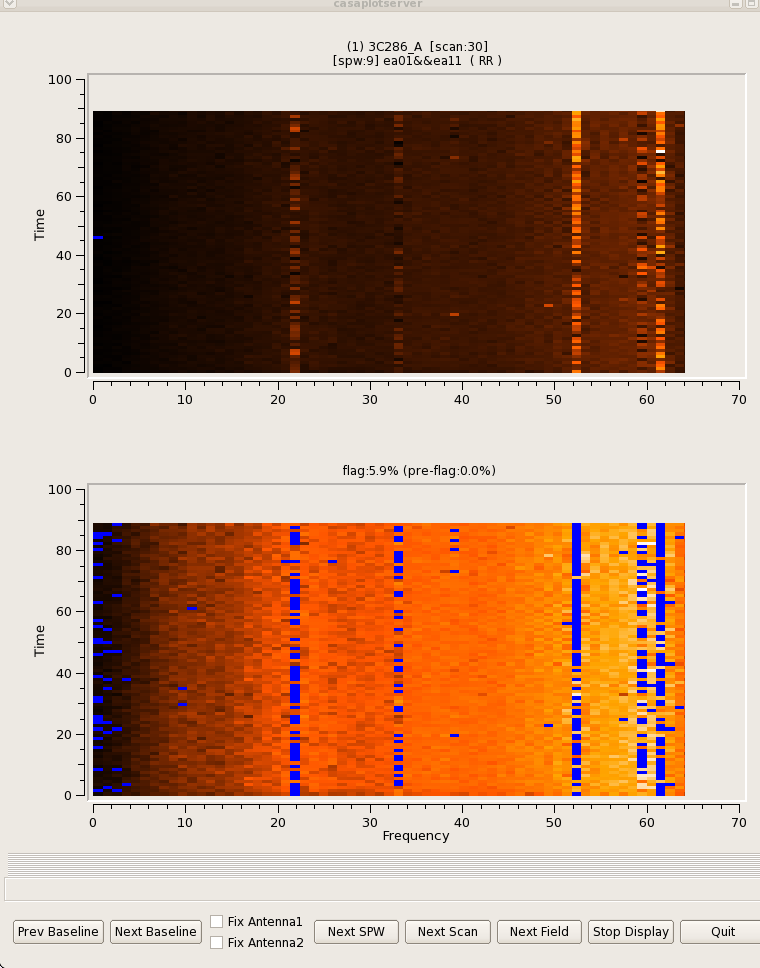
\includegraphics[scale=0.4]{flag.protect.specline.1.png}
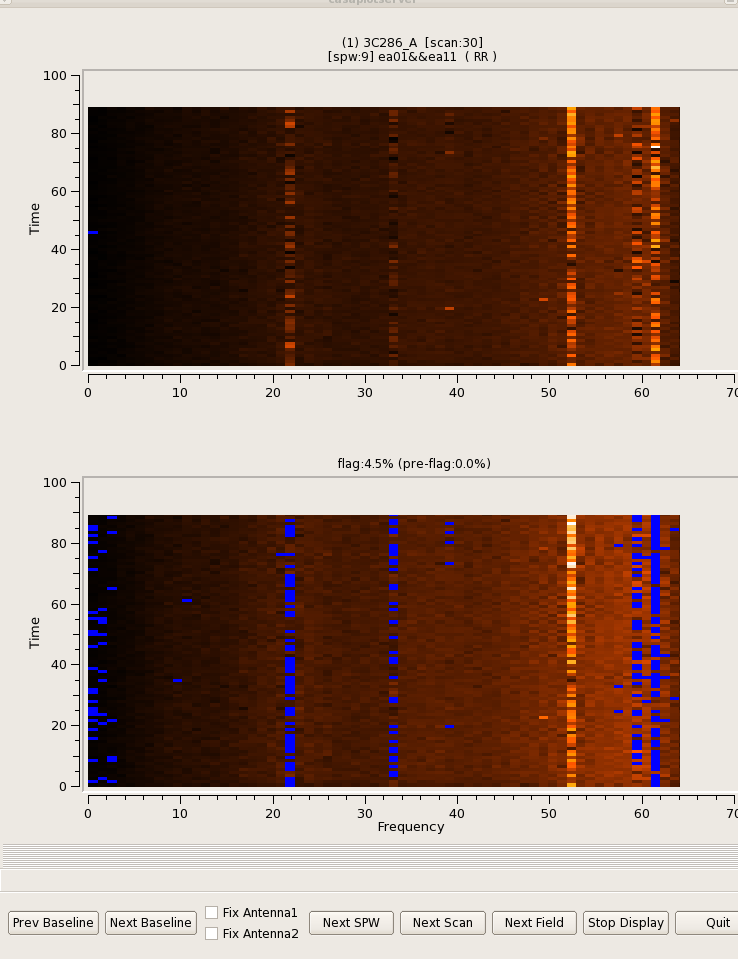
\includegraphics[scale=0.4]{flag.protect.specline.2.png}
\caption{LEFT : This screenshot represents a run where 'tfcrop' was run on a spw='9' with mainly narrow-band RFI.  RIGHT : An example of protecting a spectral line (in this case, demonstrated on an RFI spike) by setting the spw-selection to spw='0:0~45;53~63'.   In both figures, the top row indicates the data before flagging, and the bottom row after flagging.}
\end{figure}

{\red
FIG2 : Broad-band RFI
}



%%%%%%%%%%%%%%%%%%%%%%%%%%%%%%%%%%%%%%%%%%%%%%%%%%%%
%%%%%%%%%%%%%%%%%%%%%%%%%%%%%%%%%%%%%%%%%%%%%%%%%%%%


\subsection{List of flag commands (flagdata, flagcmd)}
\label{Sec:FlagCmdLists}
There are two flagging tasks in version 4.0 of CASA. The main task flagdata is
a replacement for the old flagdata/flagdata2/testautoflag/flagautocorr. This
task can take parameters input from the interface as well as input from an
external text file or a list of strings. This is the so-called list mode. All the flagging commands
that apply to an MS can be combined into one single text file and read in for
processing. Similarly, the flagging commands can be written in a Python list of strings
and passed in the command line to the task. Only the summary mode is not allowed in list mode to avoid
confusion when several summaries are present in the list. The user can run
flagdata separated to get the summary of the list. 

The other task, flagcmd is a replacement for the previous version of flagcmd. It
has a re-factored interface and it can do much more than the previous version.
All the flagging modes available in flagdata are also allowed in flagcmd
(except again for the summary mode). Several input modes are available: table,
list and xml. Actions to perform on the input are: apply, unapply, list,
clear, plot and extract.


\subsubsection{Flag Reports/Views}

Here are some examples of flag report displays on two datasets.
\begin{enumerate}
\item Percentage of data flagged vs frequency : To assess how much usable data is present in each spectral-window, for later processing, and imaging sensitivity-estimates.
\item Percentage of data flagged vs antenna-position : To assess whether the RFI is restricted to only some antennas and therefore may be local.
\item Percentage of data flagged vs baseline-length : To assess expected sensitivities for different spatial scales, since local RFI correlates better on shorter baselines than longer ones.
\end{enumerate}

